\documentclass[12pt,letterpaper]{article}
\usepackage[margin=1in]{geometry}
\usepackage{fancyhdr}
\usepackage[utf8]{inputenc}
\usepackage{palatino}
\usepackage{microtype}
\usepackage{hyperref}
\usepackage{graphicx}
\usepackage{lastpage}
\usepackage[hang,small,margin=1in]{caption}
\usepackage{titlesec}

\renewcommand{\headrulewidth}{0pt}
\fancyfoot{}
\fancyfoot[C]{\sffamily Page \thepage\ of \pageref{LastPage}}
\pagestyle{fancy}

\titleformat{\section}{\bfseries\MakeUppercase}{\arabic{\thesection}}{1em}{}
\titleformat{\subsection}{\bfseries}{\arabic{\thesection}.\arabic{\thesubsection}}{1em}{}
\titleformat{\subsubsection}{\itshape}{\arabic{\thesection}.\arabic{\thesubsection}.\arabic{\thesubsubsection}}{1em}{}

\setlength{\parindent}{0cm}
\setlength{\parskip}{1em}

\captionsetup[figure]{labelfont=it, font=it}
\captionsetup[table]{labelfont={it,sc}, font={it,sc}}

\hypersetup{colorlinks, linkcolor = black, citecolor = black, urlcolor = black}
\urlstyle{same}



\begin{document}

\fancyfoot{}
\begin{center}
    \hfill \\
    \vspace{4in}
    {\bf\Huge CS457 Project \#5 \\}
    \vspace{2in}
    {\Large Soo-Hyun Yoo \\ February 11, 2015}
\end{center}

\newpage
\fancyfoot[C]{\sffamily Page \thepage\ of \pageref{LastPage}}

\section*{Source Files}

\begin{itemize}
    \item p5.glib
    \item p5.vert
    \item p5.frag
\end{itemize}


\section*{Explanation}

\subsection*{p5.glib}

We put ourselves in perspective mode, place the eye at positive Z, and point
the camera at the origin with positive Y as the up vector.

We declare the vertex and fragment files to be used as well as some variables
to display in sliders. We set a default color and initialize an object.

\subsection*{p5.vert}

We calculate the sine wave displacement, noise, and various lighting vectors in
the vertex shader.

First, we declare the normal, light, and eye vectors as outputs, as these will
be used by the fragment shader to calculate the pixel color. Uniform variables
are then declared.

A {\tt RotateNormal} function is defined that takes two angles and a vector to
rotate and outputs the normalized rotated vector. It does this by calculating
sines and cosines of the input vector and adding or subtracting them to the
appropriate vector components. Normalization shrinks the vector back to length
1.

In the main function, we recalculate the Z position using the X and Y positions
and the sine function. The sine displacement can be started from different
Y positions at variable amplitude and frequency.

Noise is calculated using the same X, Y, Z coordinates and the user-specified
amplitude and frequency.

Surface tangents in the X and Y directions are calculated in order to
approximate a normal vector via a cross product.

Finally, lighting vectors are calculated from the normal vector estimate (and
rotated) and the user-specified light position.

\subsection*{p5.frag}

We declare the input vectors and uniform variables.

If the alpha channel is 0, the pixel is discarded.

The ambient, diffuse, and specular colors are calculated from the
user-specified color parameters. The RGB channels of these three are combined
with the user-specified alpha value to produce the output pixel color. Note
while the three colors are {\tt vec4}s and thus could simply be added, having
a user-specifiable alpha value makes it easy to fiddle with the transparency.

\newpage
\section*{Results}

\begin{figure}[!h]
    \centering
    
\includegraphics[width=1.0\textwidth]{img/plain.png}
    \caption{Default shape}
\end{figure}

\begin{figure}[!h]
    \centering
    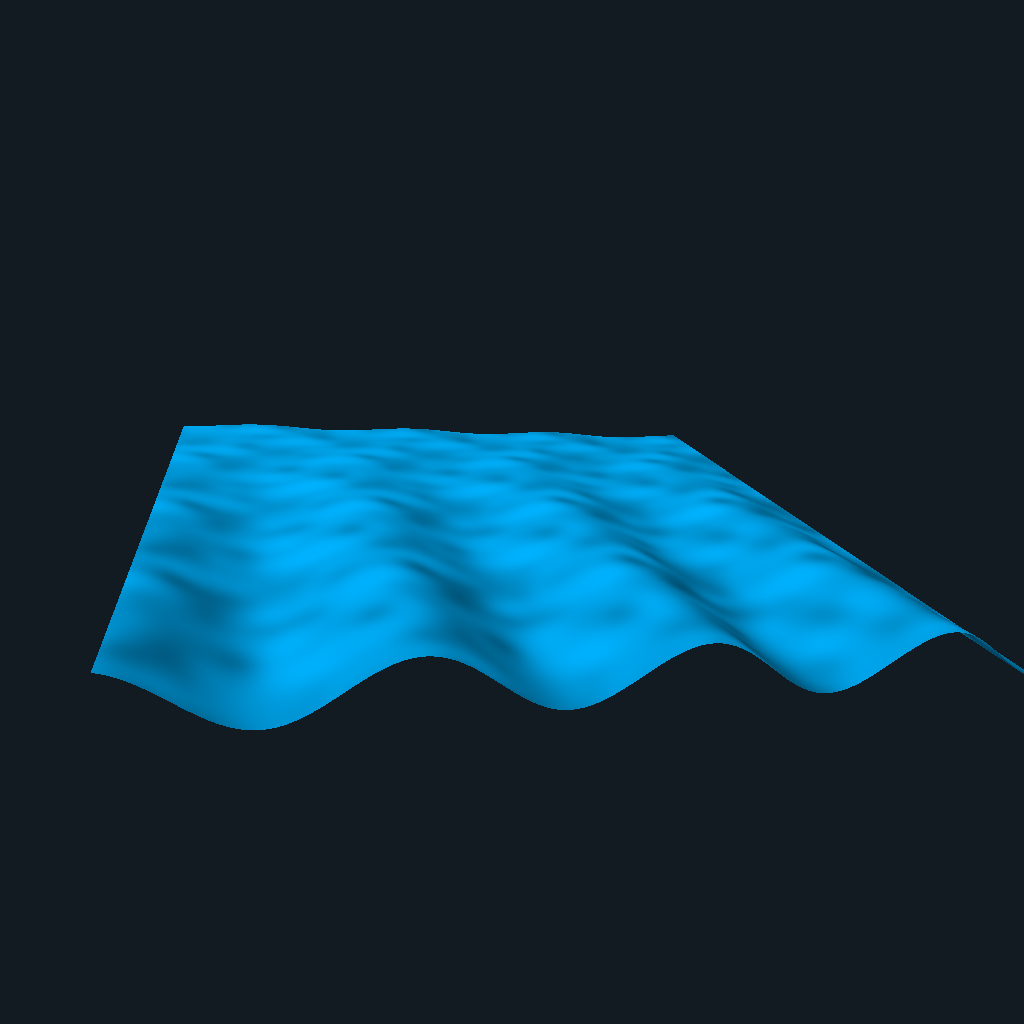
\includegraphics[width=1.0\textwidth]{img/small_k.png}
    \caption{Small K}
\end{figure}

\begin{figure}[!h]
    \centering
    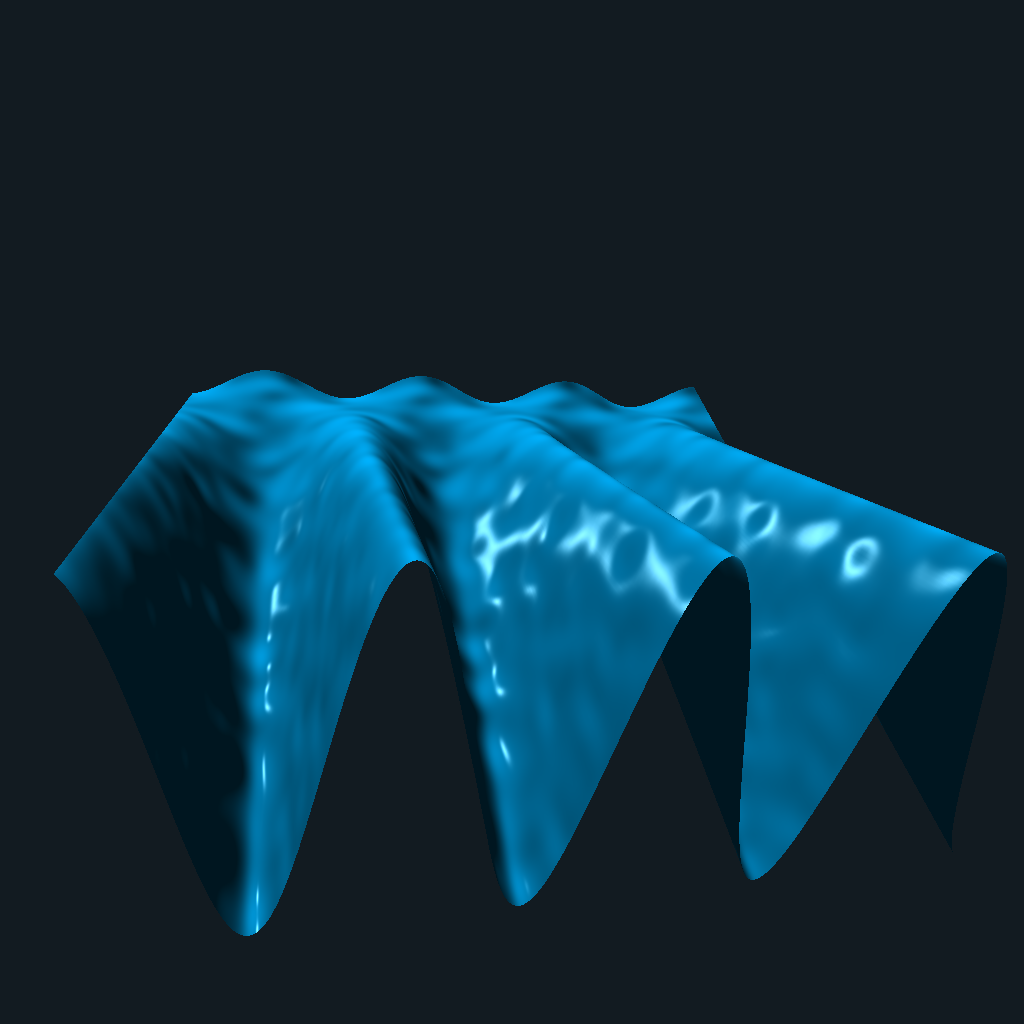
\includegraphics[width=1.0\textwidth]{img/large_k.png}
    \caption{Large K}
\end{figure}

\begin{figure}[!h]
    \centering
    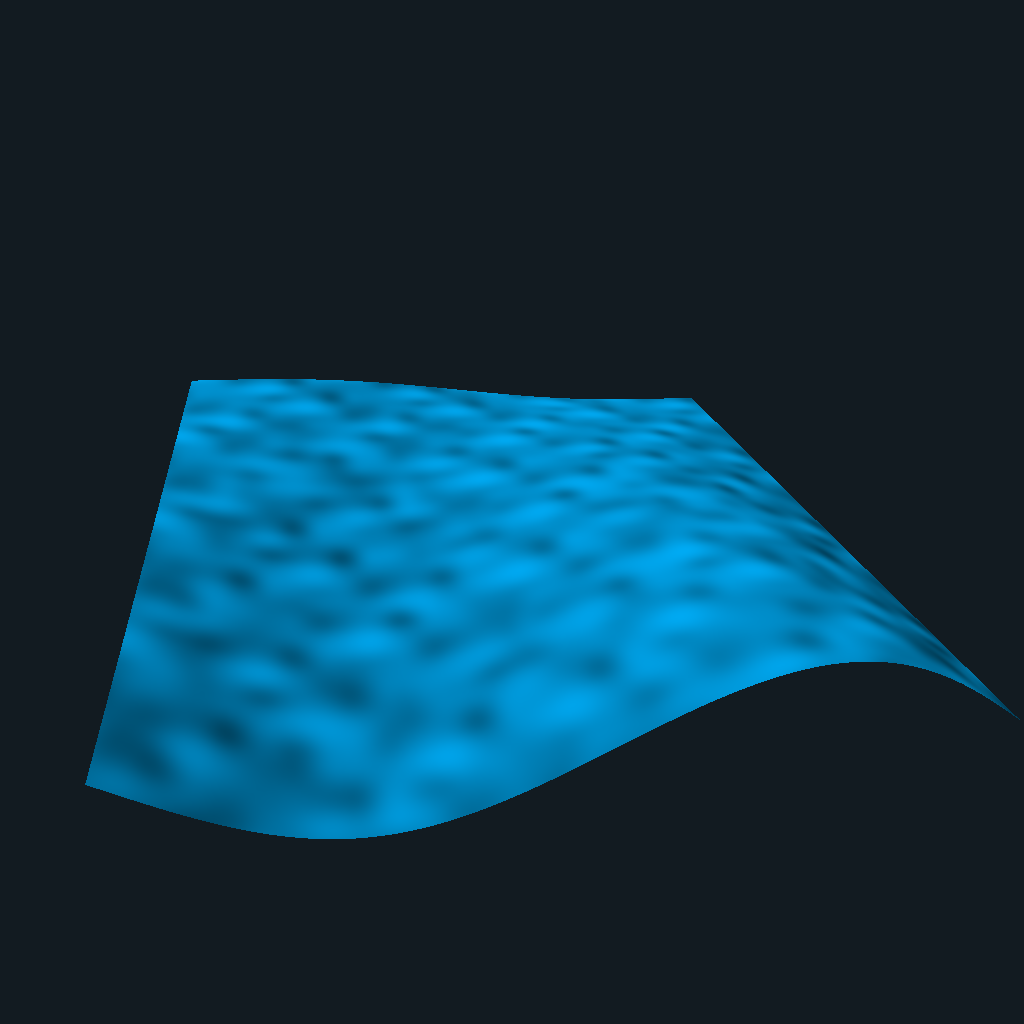
\includegraphics[width=1.0\textwidth]{img/larger_p.png}
    \caption{Larger P}
\end{figure}

\begin{figure}[!h]
    \centering
    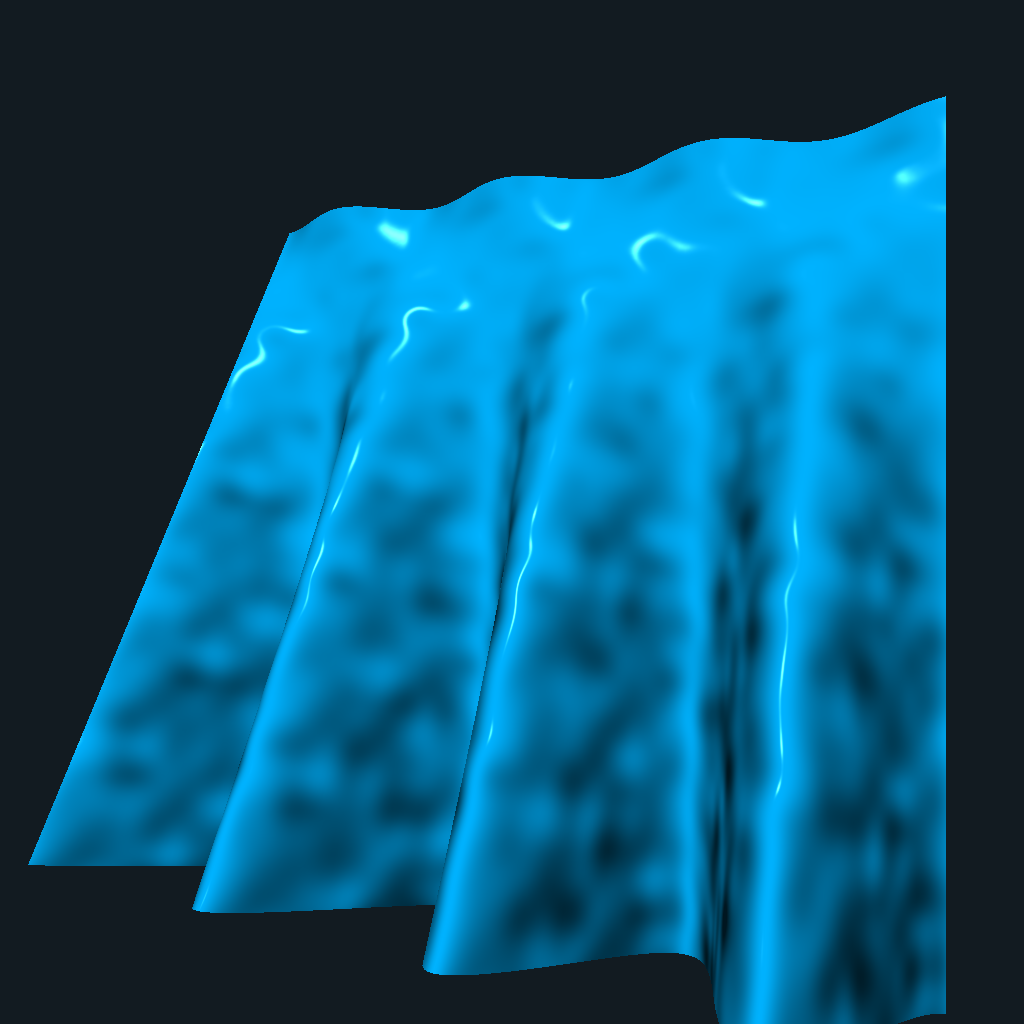
\includegraphics[width=1.0\textwidth]{img/bump_shiny.png}
    \caption{Bump mapped and extra shiny}
\end{figure}

\end{document}
